
\section{Aufbau}
\label{sec:Aufbau}

Im ersten Teilversuch wird für die Fourier-Analyse mittels Fourier-Transformation wie in Abbildung \ref{fig:Aufbau1} dargestellt das Signal eines Funktionsgenerators auf einen Analog-Digital-Konverter gegeben, sodass mithilfe eines Rechners die Fourier-Transformation durchgeführt werden kann. Das entstehende Frequenzspektrum wird an einem Oszilloskop ausgegeben. Da der Analog-Digital-Konverter nur diskrete Messwerte liefert, muss die Abtastfrequenz $\omega_.A$ das Abtasttheorem
\begin{equation}
\omega_.A > 2\omega_.{max} = 2n\omega_.1
\end{equation}
erfüllen, da sonst die Funktion $f$ nicht rekonstruiert werden kann. Dabei ist $\omega_.1$ die Grundfrequenz und $n$ die $(n-1)$te Oberwelle.

\begin{figure}
	\centering
	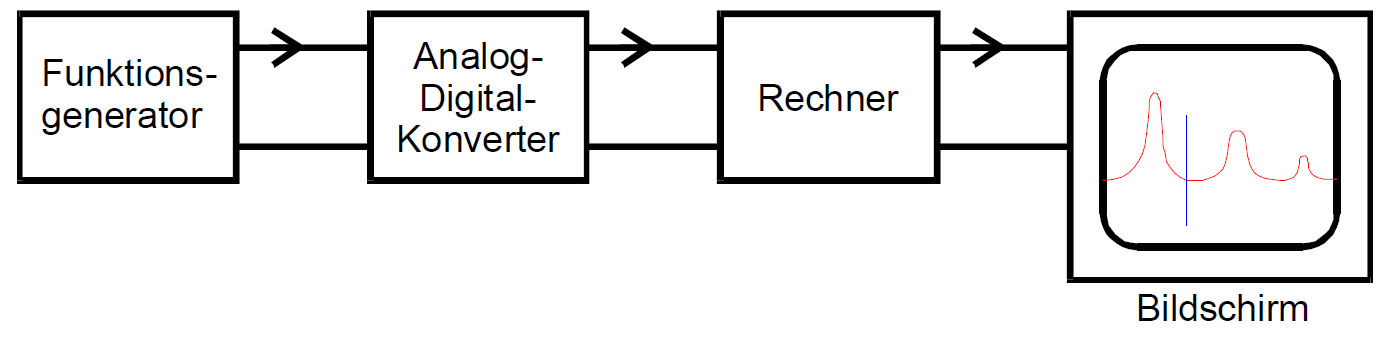
\includegraphics[width=\linewidth-75pt,height=\textheight-75pt,keepaspectratio]{content/images/Aufbau1.png}
	\caption{Der Versuchsaufbau für den ersten Teilversuch\cite{V351}}
	\label{fig:Aufbau1}
\end{figure}

\newpage
\noindent Im zweiten Teilversuch wird für die Fourier-Synthese ein Signalgenerator verwendet, der Sinusschwingungen mit einem vielfachen der Grundfrequenz liefert, die einzeln aufaddiert werden können. Die Amplituden der einzelnen Schwingungen sind verstellbar und die Phasen konstant. Dabei müssen Die Phasenverschiebungen bei geradem oder ungeradem $f(t)$ die Werte $0$ oder $\pi$ annehmen.  
Das Ausgangssignal wird mit einem Oszilloskop sichtbar gemacht.